\documentclass{njubachelor}
\usepackage{algorithm}
\usepackage{algorithmic}
\usepackage{listings}

\sid{14108416} %学号
\cauthor{姜永铭} %学生姓名
\ctitle{基于基因表达谱特征选择方法研究} %题目
\cdepartment{卓越学院} %院系
\cspecialization{软件工程} %专业
\cmentor{葛瑞泉}{讲师} %指导老师 职称
\ckeywords{} %关键词
\cdate{2018.6.9} %提交日期

\begin{document}

\makectitlepage

\pagenumbering{Roman}
\thispagestyle{plain} %该页一般无页眉
\vspace*{0em}

\maketoc

\newpage
\pagenumbering{arabic}

\thispagestyle{plain} %该页一般无页眉

\section{绪论}

2017年2月,国家癌症中心发布了中国最新癌症数据,汇总了全国347家癌症登记点的数据.中国癌症统计一般滞后3年,最新公布的是2013年的发病和死亡数据.与2012年相比,癌症新发人数继续上升,从358万增加到368万,增幅3\%;每天约有1万人诊断癌症,每分钟约有7人诊断为癌症.世卫公布的数据显示, 全球每年约有880万人死于癌症,占全球每年死亡总人数近六分之一,死者大多数在中低收入国家.每年有1400多万新发癌症病例,预计到2030年这一数字将增加到2100多万.

一般来说,治疗癌症的方案大抵相同。可靠并精确诊断出癌症是有效治疗癌症的基础。癌症的诊断目前属于临床医学的范畴,通过一系列的射线照射比如X光来发现癌变的细胞,但这种方法准确率低,而且X光本身具有辐射,会造成染色体异常,反而还会造成细胞癌变。目前临床上比较靠谱的癌症细胞检测的方式就是进行活体组织检查,通过从患者体内切取、钳取或穿刺等方式去除病变组织,进行病理检测。活检的一个最大弊病就是如果被检测细胞是良性肿瘤,在穿刺的时候会扎破良性肿瘤的包膜,从而造成癌细胞的大面积扩散。传统临床医学是以组织形态学为基础,往往对组织形态相似的癌变组织作出错误的判断,无法达到应有的治疗效果,影响病情的治疗,最终可能导致死亡。

面对如此高涨的癌症发病率,全球抗癌研究“多路提速”.中国、美国等国都加大了对抗癌研究的支持力度.各国研究人员正争分夺秒在基因组学、免疫疗法、基因编辑等方面寻求抗癌新突破.

基于高通量的基因芯片技术的出现,随着生物技术也在飞速的发展,基因探针技术的应用,从分子生物学的角度研究癌症提供了可能. 研究人员研究的角度多了一个维度,由于分子层面更能表达生物的信息,大量的使用表明,癌症的发生和发展与相关标志物基因的表达异常相关。因此从分子角度研究癌症比传统临床医学的准确率可以大大提高。

如何挖掘这样与癌症相关标志物基因的生物数据也是生物信息领域的重点研究方向。虽然数据挖掘和机器学习的理论日渐完善,相关技术也应用广泛,但是针对生物数据独有的一些显著特征,仍有很多问题需要我们去一点一点的解决。目前来看,检测成本较高、癌症疾病取样困难,导致总体样本的数量很少,但是癌症基因表达谱特征数据又属于一个高维特征数据集,这样就出现了小样本大特征的情况,这在机器学习和数据挖掘领域被称为“大p小n”问题。如果处理这样的“大p小n”的数据,避免维度灾难的发生,是基因表达谱数据分析中的核心问题。

癌症发病数字看起来虽然悲观,但是并非不可预防.这里,我打算用统计学方法,利用机器学习的手段,借助计算机,根据基因表达谱特征来预测癌症的发病情况.以此来提早预防癌症,做到早发现早治疗,减少癌症给人们的健康、经济带来的困扰.

\section{国内外研究现状}

\subsection{需求分析}

1)基因探针的技术不断发展,会产生大量的生物数据.但是我们对于纷繁复杂的数据,我们很难从中知道这样的数据表达是怎么的信息.那么,如何从这样纷繁复杂的数据中获取到有效、精准的信息,是生物医学界面临的重要问题.

2)由于基因探针技术成本的问题,获取到的数据虽然维度很高,但是样本数并不是很多,同时,特征之间的具有高复杂度、高噪声的特点.这样的数据在机器学习领域称为“大p小n”问题.对于这样的生物数据如果所有的特征都用在分类或者回归模型当中,一定会产生过拟合现象,所以在做分类和回归问题之前要从高维特征中提取最具有代表性、最具有价值的特征组合。 针对某个癌症基因表达谱数据,一般只有少量的特征与分类结果强相关,大部分特征数据是冗余或者无效甚至负相关的,如何有效的从海量特征数据中去除冗余、无关和负相关的特征,进而提取出与病症强相关、有效的特征也是本研究要关注和亟需解决的很重要的问题.

\subsection{国内外研究现状}
目前,对于基因表达谱数据特征选择方法研究一般是按照特征子集的评价和策略对特征方法进行研究.但是这样的研究方法并没有考虑到特征之间的复杂度,对于这样高维的数据特征和特征之间,特征和类标之间存在着一定关系.在保证特征子集高评价的条件下,去除掉冗余特征,选择出特征间高独立性的特征也是本研究主要做的事情.

目前,对于基因表达谱数据特征选择方法研究主要是按照特征子集的评价和策略对特征方法进行研究.对于特征选择大致分为三种方法:过滤法(filter),包装法(wrapper),和集成法(embeded).

    (1)过滤法

主要的思想就是对每一维特征赋予权重,然后根据权重进行排序,选取排在前面的一些特征作为最终的特征列表.这些过滤式特征方法虽然简单,但是只考虑了单个特征的分类能力,忽略了特征之间的关系,得到的特征列表存在冗余,从而影响分类的准确性. 过滤法的主要方法有:方差选择法,卡方检验法,信息增益和相关系数等.

1999年,Golub等用“信噪比”作为特征排序的度量来解决癌症基因表的分类问题,开创了分子级别诊断的新领域. Callow等人提出了双样本T-test特征选择方法,目的在于剔除无关特征.Hall, Mark A 在机器学习领域提出了基于相关性的特征选择(Correlation-based Feature Selection, CFS)算法,假设特征子集间相互独立,特征与类标相关性高,具有良好的实际应用表现价值.2004年Yu 和 Liu提出了基于相关性的快速过滤算法(Fast Correlation-based Feature Selection, FCBF),其优势在于能在一堆冗余特征中,保留与目标相关性更高的特征.

    (2)包装法

包装法会根据目标函数,每次选择若干特征或者排除若干特征.有确定算法和随机算法两种.

    确定算法的优势在于简单,计算开销小,但是它更容易稳定在局部最优处,有过拟合风险,依赖分类器选择特征.方法有序列化前向选择算法(Sequential Forward Selection, SFS),序列化后向删除(Sequential Backward Elimination,SBE).

随机性算法可以更少趋向稳定在局部最优,但是它的计算开销大,与确定性算法相比更容易过拟合.方法有模拟退火(Simulated Annealing),遗传算法等.

    (3) 集成法

    其主要思想是,在确定模型的过程中,挑选出那些对模型的训练有重要意义的属性.与包装法相比,嵌入法可以取得相似的性能,并大大降低时间开销.
   
    主要方法有,正则化,包括L1正则的Lasso回归,和L2正则的Ridge回归,以及决策树算法和深度学习算法.

\subsection{面临问题}
在全方面考虑特征直接的关系以及对最终评价的影响,在不考虑性能和事件复杂度的情况下,最好的方案就是枚举出所有的情况下的特征子集,对每一种情况的特征子集进行评价,然后选出评价最优的,特征数最少的特征子集。然而,对于生物的基因表达谱特征数据来说,每个数据集都是有上万个甚至更多个特征。那么,其拥有的特征子集数量就是  个,如此海量数据的计算,对于计算机的CPU计算能力和内部存储空间都是极大的挑战,即时间、空间复杂度都很高。指数级增长的计算量,对于一般计算机就是不可能完成的任务。那么如何有效地减少候选特征子集的数量,节省计算资源的消耗,是本研究要解决的第一个问题。

对于 $2^n(n > 10000)$这样数量级的数据,即使是单机计算能力再高也很难在短时间得到结果。对于单机痛点自然而然想到的就是并行处理解决方案,那么如何利用多台计算机并行计算,以及单台计算机内部多线程并行计算已达到充分利用资源的目的,同时由并行异步带来的数据不一致问题是也是本研究要解决的重要问题。

\section{相关技术}
\subsection{方法介绍}
本研究中使用的方法旨在于通过前项搜索来扩充目标特征子集.本研究使用Logistics 回归算法来评价特征自己的性能表现.我们也与其他六种特征选择选举进行了比较,他们是RRF, RFE, WRank, TRank, CFS 和 FCBF,然后从分类准确率和特征子集中特征的个数两个角度,来描述我们研究算法的优势.
\subsection{相关算法}
1) T-Rank

基于特征过滤的 T 检验算法是用在度量两个特征间差异性的最常用的方法. 它能估计两个组直接的差异性和给定统计显著测量方法的变化.

2)W-Rank

基于特征过滤的 W 检验算法计算两个样本类别直接特征差异程度的非参数化评价,并且以其鲁棒性而闻名.

3)CFS

CFS 是一个经典的特征选择算法,它对单个特征的风险评估在每个类别中扮演重要的作用.然后我们可以得到最终的特征子集.评估的方法如下 
$$M_s = \cfrac{kr_{cf}}{\sqrt{k+k(k-1)r_{ff}}}$$

$M_s$ 是含有 $k$ 个特征子集 $S$ 的评价.

$r_{cf}$ 是类标和特征之间的平均相关性.

$r_{ff}$是特征与特征之间的平均相关性.
 
4)SVM-RFE

SVM-RFE是一个基于SVM的顺序后向特征选择算法.它首先训练模型,然后给每个特征打分,剔除掉分数最低的特征.然后再用剩下的特征接着训练模型.最后,直到选择出你需要的特征.

5)RRF

随机森林(RRF)有一个重要的特点:它可以计算单个特征的重要程度.所以我们可以根据每个特征的重要程度进行排序,然后选择重要性最高的特征子集.

6)FCBF

基于相关性的快速过滤算法(FCBF)是一个基于对称不确定性(SU)的快速特征选择算法.

首先,我们计算每个特征 $F_i$ 与目标变量 $C$ 直接的相关性.
$$SU(X,Y) = 2\cfrac{IG(X,Y)}{E(X)E(Y)}$$

然后,我们选择出那些相关性高于阈值的特征,然后降序排序 $SU_{F_{i,c}}$并且计算每个特征和其他小于  $SU_{F_{i,c}}$ 的特征之间的相关性.
最后,我们选择出那些  $SU_{F_{i,j}}$ 高于 $SU_{F_{i,c}}$ 的特征 $F_j$.

\subsection{评价指标}
评价一个二分类模型的分类能力有一些指标,如:准确率(Accuracy),召回率(Recall),精确率(Precision),特异性(Specifity) 和 F1 等等.

混淆矩阵(Confusion Matrix): 混淆矩阵是一种特定的用来呈现算法性能的可视化效果的矩阵.混淆矩阵是用来反映某一分类模型的分类结果的,其中行代表的是真实的类,列代表的是模型的分类.


如图1 所示,这里有4个指标,分别是正确的正样本(true positive,TP),错误正样本(false positive, FP), 错误负样本(false negative,FN),正确负样本(true negative, TN).

TP是被预测为正例的正样本.

FP是被预测为正例的负样本.

FN是被预测为负例的正样本.

TN是被预测为负例的负样本.

综上,我们有 $P = TP + FN$ 和 $N = TN + FP$.

分类的表现力被定义为:

1)准确率(accuracy):	准确率是最常用的分类指标,它的值为正确预测的正反例数/总数
$$Accuaracy = \cfrac{TP+TN}{P+N}$$                                 

2)召回率(recall):召回率表现出在实际正样本中,分类器能预测出多少。与真正率相等,可理解为查全率
$$Recall = \cfrac{TP}{TP + FN}$$        

3)精确率(precison):精确率容易与准确率混为一谈。其实,精确率这是针对预测正样本而不是所有预测正确的样本。表现为预测初始正的里面有多少是真正的真。可理解为查准率
$$Precision = \cfrac{TP}{TP+FP}$$
                                       
4)F1 score:F1值是精确率和召回率的调和值,更接近与两个数较小的那个,所以精确率和召回率接近时,F值较大。很多推荐系统的评测指标就是用F1值。
$$F1 = \cfrac{2\times Precision \times Recall}{Presion + Recall}$$

5)特异性(specificity):特异性反映了分类器检验负样本的能力
$$Specificity = \cfrac{TN}{TN+FP}$$

\section{算法设计}
\subsection{算法简介}
对于高维数据进行降维处理,一般有两种方式。一种是维度的转换,如PCA、SVD等等,另一种是选择特征。对于本研究,特征选择在不改变原始数据特征的情况下,能更好的对模型进行一个生物的解释。

利用最大信息系数进行过滤:

信息论中一个重要的概念是熵——这是一个衡量给定概率分布的不确定性的度量。概率分布描述了与特定时间相关的一系列给定结果的概率。
$$H(x) = -\sum^N_{k=1}P(X=k)\log_2P(X=k)$$

交叉熵是熵的一个拓展概念,它引入了第二个变量的概率分布.
$$H(X,Y)=-\sum_{k=1}^NP(X=k)\log_2P(Y=k)$$

两个相同概率分部之间的交叉熵等于其各自单独的熵。但是对于里欧昂个不同的概率分布,他们的交叉熵可能跟各自单独的熵有所不同。这种差异可以叫做散度,可以通过KL散度(Kullback-Leibler divergence)量化得出,其用途之一是计算两个变量的互信息(MI). 

互信息可以定义为:连个随机变量的连个分布和边缘分布之间的KL散度。如果而知相同,MI取值为0.  如果不同,MI值就为一个正数,二者之间差异越大,MI值就越大. 

对于两个离散随机变量X 和 Y 的互信息可以定义为:
$$I(X;Y) = \sum_{y\in Y}\sum_{x\in X}p(x,y)\log\left(\cfrac{p(x,y)}{p(x)p(y)}\right)$$

对于两个连续性随机变量 X 和 Y,则定义为:
$$I(X,Y) = \int_y\int_xp(x,y)\log\left(\cfrac{p(x,y)}{p(x)p(y)} \right)dxdy$$

最大信息系数(MIC)于2011年提出,它是用于检测变量之间非线性相关性的最新方法。用于进行 MIC 计算的算法将信息论和概率的概念应用于连续型数据。

这是在给不同类型的同样“嘈杂”的关系指派类似评分时的一种可在数据中发现范围极端广泛的关系类型的统计方法。 研究人员因此在无需任何先前的对他们在寻找何种关系类型有所了解的情况下可用它来检测由多种因素驱动的复杂模式。 

MIC所依据的理念是,如果两个个变量之间存在着一种关系,那么就应该有一种方法在那些变量的散点图上画一个网格,使得大多数的数据点集中在该网格的几个单元格中. 通过搜寻这种“最适合”的网格,计算机可以计算MIC及一组可用来发现并描绘关系的相关的统计数据. 这一统计数据被称作“最大的基于信息的非参数性探索” 或MINE,它可以用来衡量两个变量间的线性或非线性的强度。

MIC度量具有普适性,它不仅可以发现变量间的线性函数关系,也可以发现非线性的函数关系,还能发现非函数关系。MIC度量也具有均衡性,对于相同噪声水平的函数关系或者非函数关系,MIC度量具有近似的值。所以MIC度量不仅可以用来纵向比较同一相关关系的强度,还可以用来横向比较不同关系的强度。

MIC度量计算的方法: 具有两个属性的数据点的集合分布在二维空间中,使用 $m\times n$ 的网格划分数据空间,使得落在第$(x,y)$格子中的数据点的频率作为 $P(x,y)$ 的估计,即
$$P(x,y) = \cfrac{\text{第(x,y)个网格中的数据点数}}{\text{总的数据点数}}$$

使得落在第 $x$ 行的数据点的频率作为 $P(x)$ 的估计,同理获得 $P(y)$ 的估计. 然计算随机变量 $X$、$Y$ 的互信息 $I(X;Y)$. 因为 $m\times n$ 的网格划分数据点的方式不知一种,所以我们要获得使互信息最大的网格划分。然后使用归一化因子,将互信息的值转换为 $(0,1)$ 区间之内。最后,找到能使归一化互信息最大的网格分辨率,即作为 MIC 的度量值。

$$ MIC = 
\max_{|x|*|y|<B} 
\left(
    \cfrac{
        \max_{\text{different grids}}
        \left(
            \sum_{x\in X,y \in Y} P(x,y) \log\cfrac{p(x,y)}{\sum_{x\in X}P(x,y)\sum_{y\in Y}P(xy)}
        \right)}
        {\log \min\{\|X\|,\|Y\|\}}
\right) 
$$

结合 Apriori 思想进行启发式选择

Apriori 算法的思路是由频繁(k-1)-项集生成候选k-项集,然后根据最小支持度判断该候选k-项集是否是频繁k项集。那么问题在于,如何从频繁(k-1)-项集生成候选k-项集。其实就是利用Apriori的一个性质——一个频繁项集的任一子项集也应该是频繁子项集,所以一个项集是非频繁项集,那么它的超集也应该是非频繁项集。
我们的研究也可以利用Apriori 算法的思想,通过项集来搜索出最优的特征子集,具体做法如图2所示

这里,我们以输入数据集 $F=\{A,B,C,D,E\}$ 为例,图2 的基本流程是

1)初始假设准确率的阈值 $acc_0$ 为 $0.5$,候选$1-$项集为输入数据集$F$本身,计算每个子集的分类准确率,根据阈值进行过滤.

2)得到频繁$1-$项集$M_1$之后,将准确率阈值$acc_0$更新为$acc_1 = 0.9$.

3)$M_1$与$F$做笛卡尔积,得到频繁$2-$项集,在根据准确率阈值$acc_1$进行过滤.

4)如此反复更新阈值,做笛卡尔积,直到得到我们需要那个的特征子集.


\subsection{整体流程}
如图3 所示,本研究的算法的主要流程就是先根据原始数据集生成若干特征子集,然后对特征子集进行评价,评价结果满足停止准则就下一步进行交叉验证,否则继续生成特征子集.


这里的“生成特征子集”的步骤,采用上一小结中提到的Apriori的思想,在保证算法性能的的情况下,在尽可能小的特征空间中进行结果的搜索和评价。

评价步骤,我们这里采用的逻辑斯蒂回归作为分类器进行特征子集的评价,以分类的准确率作为评价的标准。

\subsection{实验步骤}

我们的实验中使用的数据集由表1所示,一共有六个数据集,分别是Colon、ALL1、Lymphoma、CNS、Adenoma和Gastric,这些数据集包含了两千到一万个特征数,来验证不同特征个数数据集的的表现能力。


如图4所示,对于每个数据集,我们都将我们的特征选择算法MAFilter与目前业界主流的方法,例如:TRank、WRank、CFS、FCBF、RRF和SVM-Rfe,分别选出各自的特征子集。然后利用SVM、KNN等分类器进行交叉验证。进而得到最终的结论。


如图5所示,在利用MIC值选择候选集时,我们假设任意两个变量之间存在某种相关性. 首先计算特征变量 $X$ 内部两两变量之间的MIC值,形成一个二维矩阵 $A$, 然后计算特征变量 $X$ 和目标变量 $Y$ 之间MIC值,生成一个向量 $b$.然后我们设定一个阈值 $r$.

1)选取第一个特征:

选取第一个特征比较简单,只需要将比较当前特征和类标之间的 MIC 值 $b_i$ 与阈值 $r$. 如果 $b_i > r$,说明当前特征与类标之间的相关性较大,那么我们就将其加入到候选集$F_1$中.

2)选取第二个特征:

设当前待选特征为第 $j$ 个特征,遍历 $A$ 中的每一行,记为第 $i$ 行,若$a_{ij} > r$, 就说明两个特征之间相关度较低,彼此较独立,那么我们就将特征子集$\{i,j\}$,加入到候选集 $F_2$ 中.

3)选取第三个特征:

如图6所示,在候选集$F_k(k>2)$中选取每一个特征子集,记为 $H_m$. 在矩阵 $A$ 中查出 $H_m$ 任意两对特征组合的mic值,记其中最小的值为 $a_min$ .记当前待选特征为第 $i$ 个特征,找到当前特征与Hm中每一个特征间mic值的最大值,记为$max_mic$.若$max_mic < a_min$ ,则将 $\{H_m ,i\}$ 添加到 下一候选集Fk+1 中.
之后,设置一个准确率的阈值$Acc$,利用LogisticRegression算法,评价特征组合的分类效果. 对计算结果进行排序,找到准确率最高的特征组合,就是我们要找的最好的组合.

\subsection{算法伪代码}
\newpage
\begin{algorithm}
    \caption{MAFilter}
    \begin{algorithmic}[1]
        \REQUIRE ~~
        1)含有正(P) 样本和负(N)样本的二分类生物数据集.数据集的特征(F)维度为N,样本数为M;\\
        2)Mic阈值;\\
        3) 分类模型 A (默认为Logstic回归算法);\\
        4) 最大特征数 $$CutOffMaxFeatureNum$$ (默认为10)\\
        \ENSURE ~~
        准确率最高的特征子集;
        \STATE The initial set of features subset is $M_0 =\{\}$, where $M_0$ is a empty set.
        \STATE The initial set of features candidate  set is $C_0 =\{i | i \text{is index of features}\}$
        \FOR{each $i \in [0...n-1]$}
            \STATE $M_{i+1}=\{\}$
            \STATE $C_{i+1}=\{\}$
            \STATE $m = $ the size of $M_i$
            \FOR{each $j \in [0...m-1]$}
                \IF{$i<3$}
                    \STATE mic = the mic value between $X[i]$ and $y$.
                    \IF{$mic > max_mic$}
                        \STATE $C_{i+1} = C_{i+1} \cup \{i \cup C_i[m]\} $
                    \ENDIF
                \ELSE
                    \STATE $mics = $ the mic value between $X[i]$ and all the feature of $M_i$
                    \STATE $max_mic = $ max mic value between two items in $M_i$
                    \IF{$\text{any one for } mics < max_mic$}
                        \STATE $C_{i+1} = C_{i+1} \cup \{i \cup C_{i}[m]\}$
                    \ENDIF    
                \ENDIF
            \ENDFOR
            \STATE The highest accuracy is set to overall accuracy in $M_i$
            \FOR{the only featrue subset $F_S \supset M_i $}
                \STATE sdf   
            % \STATE $M_{i+1}=F_{S}\cup\f_{z}$, where $f_{z} \in F$, $f_{z} \not\in F_{S}$ and $(F_{S} \cup f_{z})$ is the best model
            \ENDFOR
        \ENDFOR
        \RETURN the feature subsut $M^{'}\subset M_1 \cup M_2 \cup \dots \cup M_n$, where $M'$ has the best accuracy.
    \end{algorithmic} 

\end{algorithm}
\newpage


\section{实验结果分析}
\subsection{实验结果数据}

我们比较了WRank、TRank、CFS、FCBF、RFE、RRF特征选择算法在支持向量机(SVM)、k-最近邻(KNN)、朴素贝叶斯(NaiveBayes)、决策树(DTree)、逻辑斯蒂回归(LR)等分类模型中的分类表现能力。如表2-表7及图7-图12所示,只有在CNS数据集上,KNN分类模型跑输WRank、RFE和RRF算法;在CSN数据集上,NaiveBayes分类模型跑平WRank特征选择算法,以及在Colon数据集上,KNN分类模型跑平WRank特征选择算法。

由此可以得出结论,我们的算法在绝大多数情况下选出来的特征子集与结果的相关度更高,其分类准确率要优于其他同类算法。这对于癌症诊断的判断至关重要。由于准确性的提高,从临床生物医学的角度来看会让医生判断病症时更加精准地判断患者的病症,真正做到提前预防,精确治疗的目的。



\subsection{不足与展望}
  为了获得到更高的准确性和更小的特征子集,本研究中牺牲了一定的时间和空间。从时间角度来看,本算法的耗时要远大于同类其他算法。大部分的时间消耗主要集中在,对于过大的候选子集中每个子集进行的表现性评价的计算。同时庞大的候选子集也占据了大量的内存空间,对计算机的存储和计算能力都是不小的挑战。未来,针对空间上的压力,可以考虑利用大数据计算框架,利用分布式集群来分摊存储上的压力;对于时间上的压力,考虑并行计算和GPU进行加速


\newpage
\pagenumbering{Roman}

\begin{thebibliography}{99}
\bibitem{citekey1} 参考文献条目一.
\end{thebibliography}

\newpage
\ack

致谢内容

\newpage
\appendix

\section{附录}
\subsection{附录A: 实验代码}
\begin{lstlisting}[language=python,numbers=left]
import numpy as np
from sklearn.linear_model import LogisticRegression
import sklearn.metrics as metrics
from minepy import MINE


class McTwo(object):
    def __init__(self,X,y,X_test,y_test,k):
        self.mic_map = np.ones((X.shape[1],X.shape[1]))
        self.mine = MINE(alpha=0.6, c=15)
        self.X = X
        self.y = y
        self.X_test = X_test
        self.y_test = y_test
        self.k = k


    def compute_mic(self,X,y):
        self.mine.compute_score(X, y)
        mic = self.mine.mic()
        return mic

    def genretate_MIC_map(self):
        for i in range(self.X.shape[1]-1):
            j = i+1
            while(j < self.X.shape[1]):
                mic =  self.compute_mic(self.X[:,i],self.X[:,j])
                self.mic_map[i][j] = mic
                self.mic_map[j][i] = mic
                j+=1
        return self.mic_map


    def create_C1(self):
        """
        Create frequent candidate 1-itemset C1 by scaning data set.
        Args:
            data_set: A list of transactions. Each transaction contains several items.
        Returns:
            C1: A set which contains all frequent candidate 1-itemsets
        """
        C1 = []
        for i in range(self.X.shape[1]):
            C1.append([i])
        return C1

    def create_Candidation(self,front_candidation,index,max_mic=0.15):
        print('begin generate candidataion:')
        result = []
        count = 0
        for i in range(self.X.shape[1]):
            for canditaion in front_candidation:
                if count % 1000 == 0 and count!= 0:
                    print('It has generated %d candidation'%count)
                if i in canditaion:
                    pass
                if index <= 2:
                        mic = self.compute_mic(self.X[:,i], self.y)
                        if mic > max_mic:
                            temp = [i]
                            temp.extend(canditaion)
                            result.append(temp)
                            count += 1
                elif index == 3:
                    mic = self.mic_map[canditaion[0]][canditaion[1]]
                    if mic > self.mic_map[i][canditaion[0]] and mic > self.mic_map[i][canditaion[1]]:
                        temp = [i]
                        temp.extend(canditaion)
                        result.append(temp)
                        count += 1

                else:
                    max_mic = 1
                    for first_index in range(len(canditaion) - 1):
                        current = canditaion[first_index]
                        last_index = first_index + 1
                        while last_index < len(canditaion):
                            next = canditaion[last_index]
                            mic = self.mic_map[current][next]
                            if mic < max_mic:
                                max_mic = mic
                            last_index += 1
                        if self.mic_map[current][i] < max_mic:
                            temp = [i]
                            temp.extend(canditaion)
                            result.append(temp)
                            count += 1
                            break
        print('end generate candidataion:')
        return result



    def run(self,min_acc=0.5):
        self.genretate_MIC_map()
        result = {}
        c = self.create_C1()
        max_acc = min_acc
        size = 0
        for key in range(self.k):
            last_c = []
            for index in c:
                X_train_sub = np.array([self.X[:, i] for i in index]).T
                X_test_sub = np.array([self.X_test[:, i] for i in index]).T
                clf = LogisticRegression()
                clf.fit(X_train_sub, self.y)
                y_predit = clf.predict(X_test_sub)
                acc = metrics.accuracy_score(y_true=self.y_test, y_pred=y_predit)
                size += 1
                if size % 200000 == 0:
                    print(size)
                if acc >= max_acc:
                    if key not in result.keys():
                        result[key] = [{
                            "acc":acc,
                            "features":index
                        }]
                    else:
                        result[key].append({
                            "acc":acc,
                            "features":index
                        })
                    last_c.append(index)
            if(key not in result.keys()):
                break
            result[key] = sorted(result[key],key=lambda item:item["acc"], reverse=True)
            max_acc = result[key][0]['acc']
            c = self.create_Candidation(last_c,key+2,0.68)
        return result[list(result.keys())[len(result.keys())-1]][0]["features"]
\end{lstlisting}
\newpage


\subsection{附录B: 图片和表格}

\begin{figure}[!ht]
  \centering
  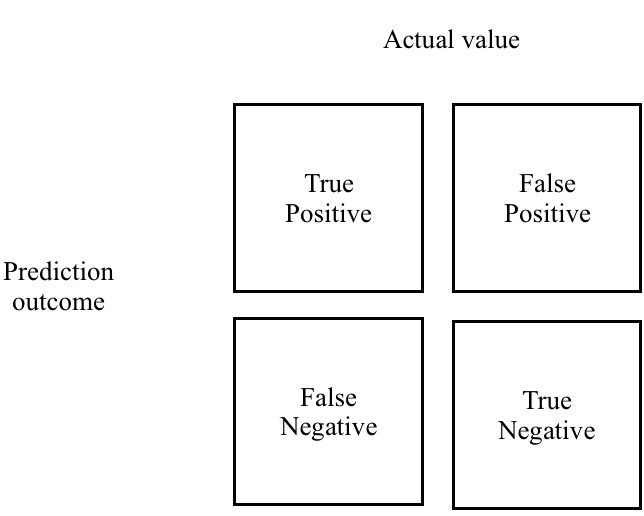
\includegraphics[width=3.5in]{pic/fig1}, 
  \caption{混淆矩阵}
\end{figure}

\begin{figure}[!ht]
    \centering
    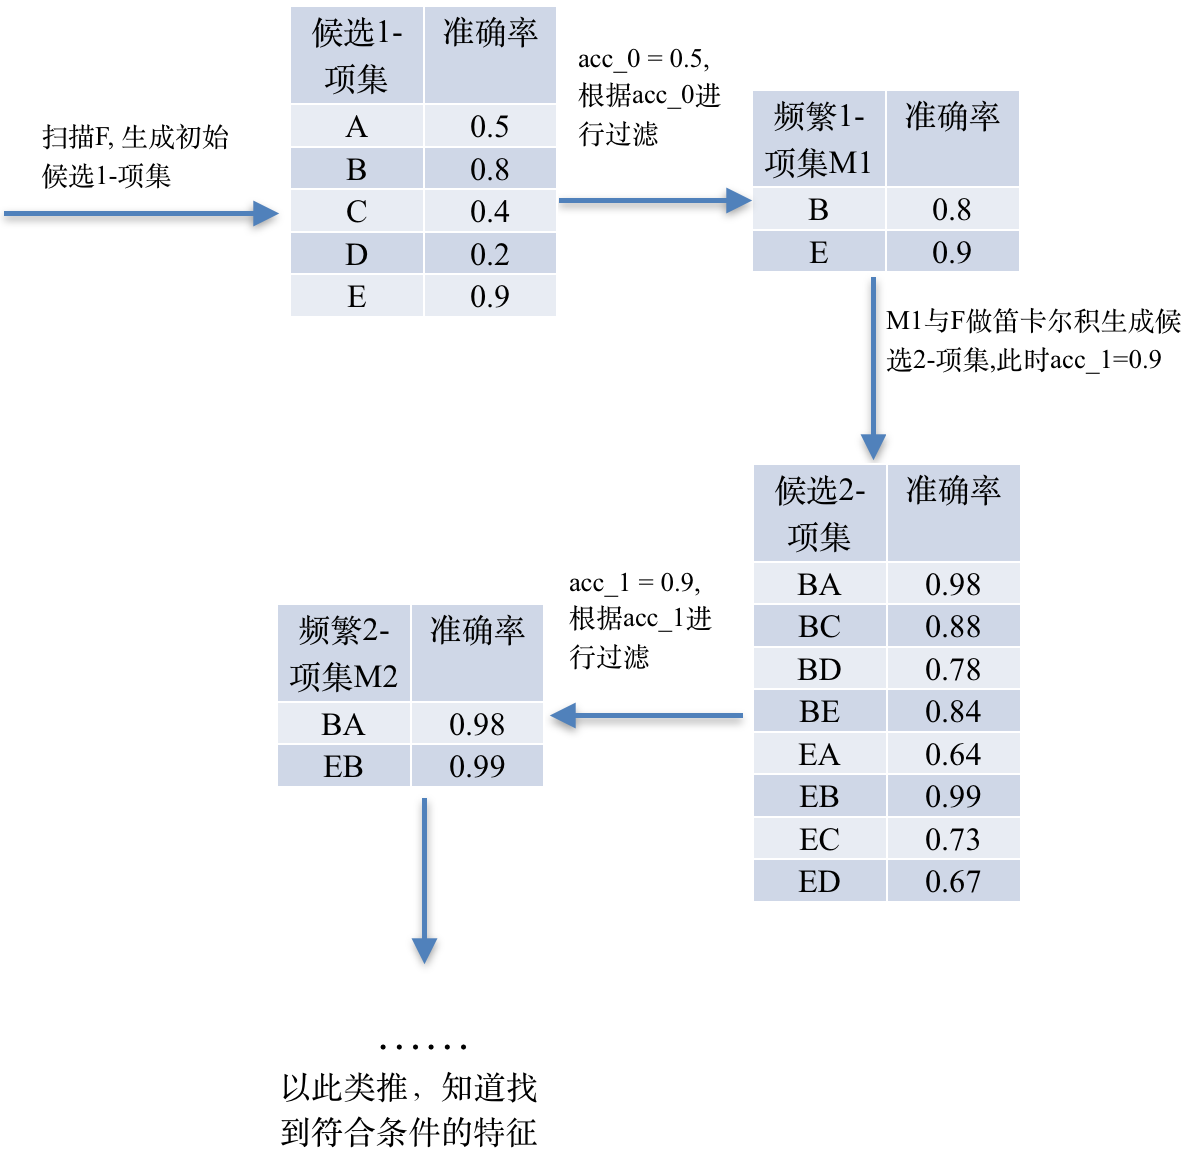
\includegraphics[width=5.5in]{pic/fig2}, 
    \caption{Apriori思想生成项集候选项集}
\end{figure}

\begin{figure}[!ht]
    \centering
    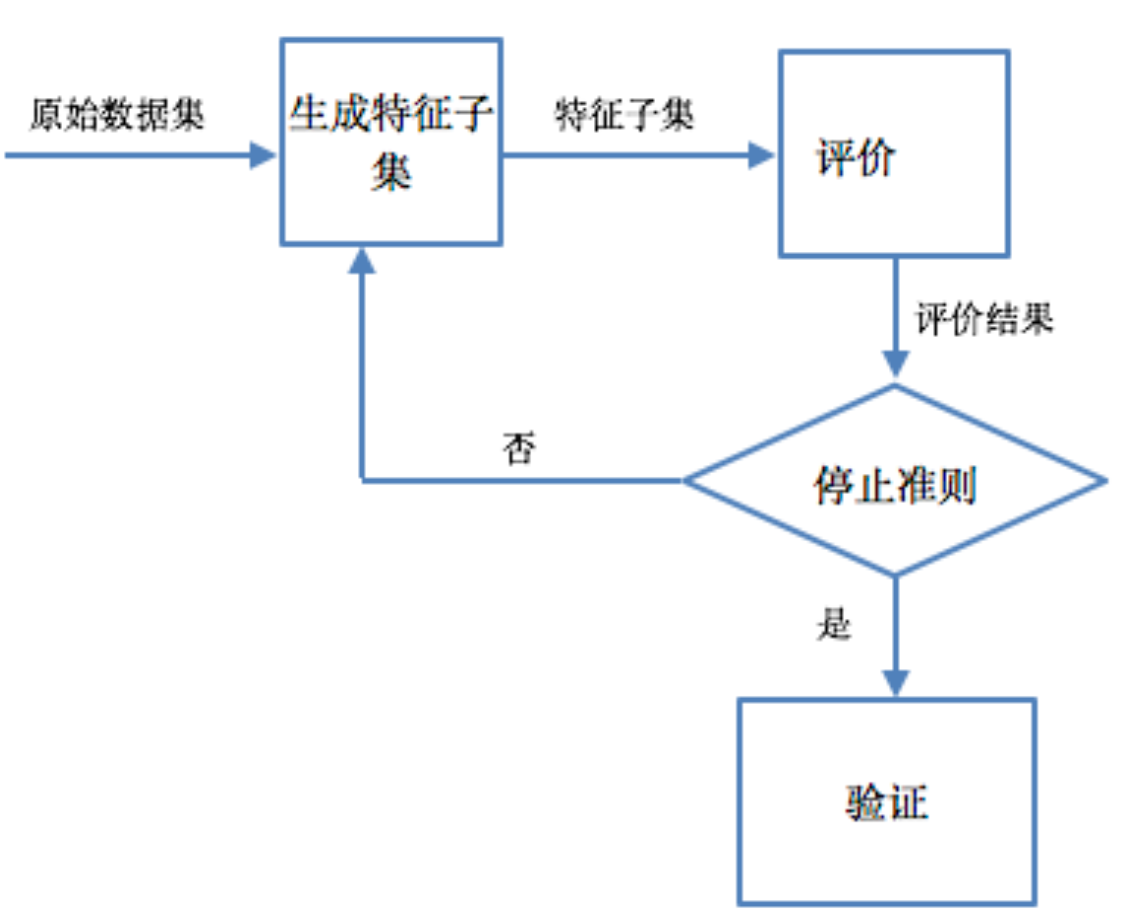
\includegraphics[width=4.5in]{pic/fig3}, 
    \caption{算法整体流程图}
\end{figure}

\begin{figure}[!ht]
    \centering
    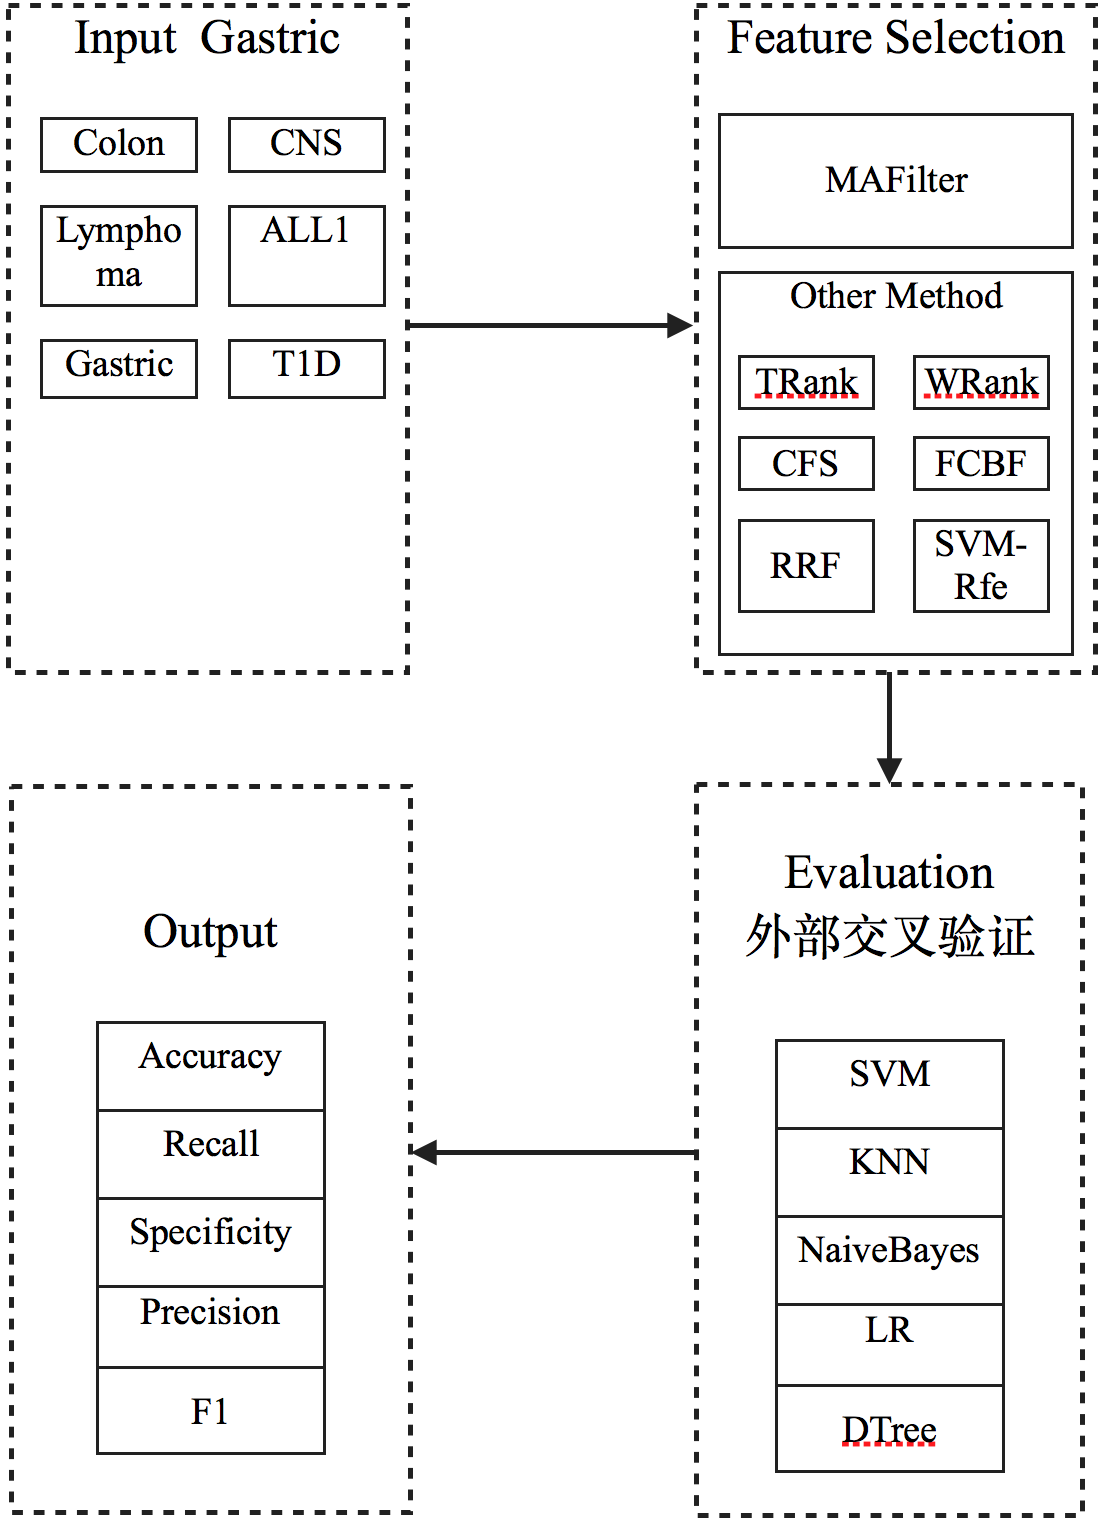
\includegraphics[width=4.5in]{pic/fig4}, 
    \caption{实验流程}
\end{figure}

\begin{figure}[!ht]
  \centering
  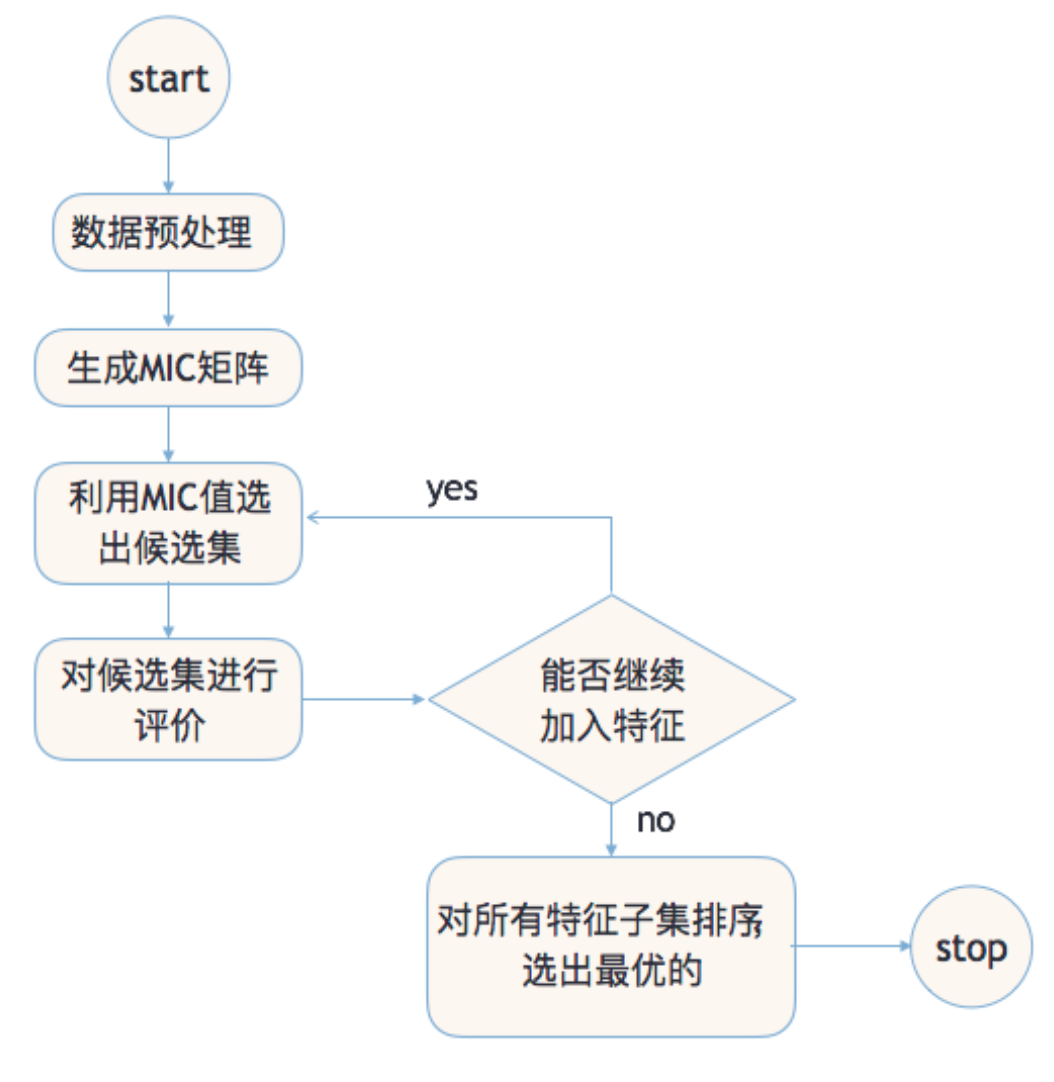
\includegraphics[width=5.5in]{pic/fig5}, 
  \caption{算法流程描述}
\end{figure}

\begin{figure}[!ht]
  \centering
  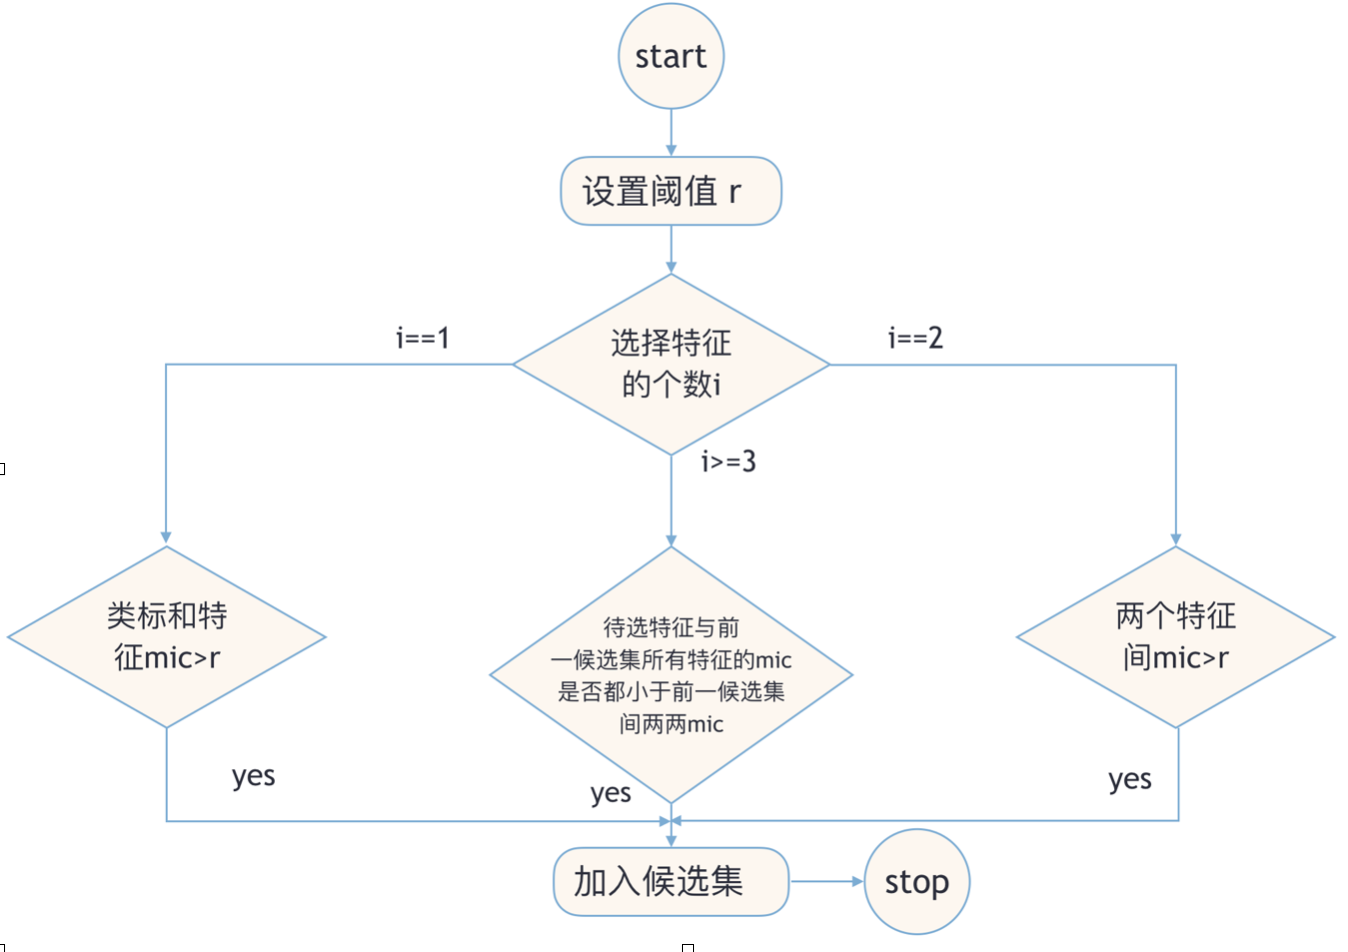
\includegraphics[width=5.5in]{pic/fig6}, 
  \caption{算法流程描述,选取三个以上特征}
\end{figure}

\begin{figure}[!ht]
  \centering
  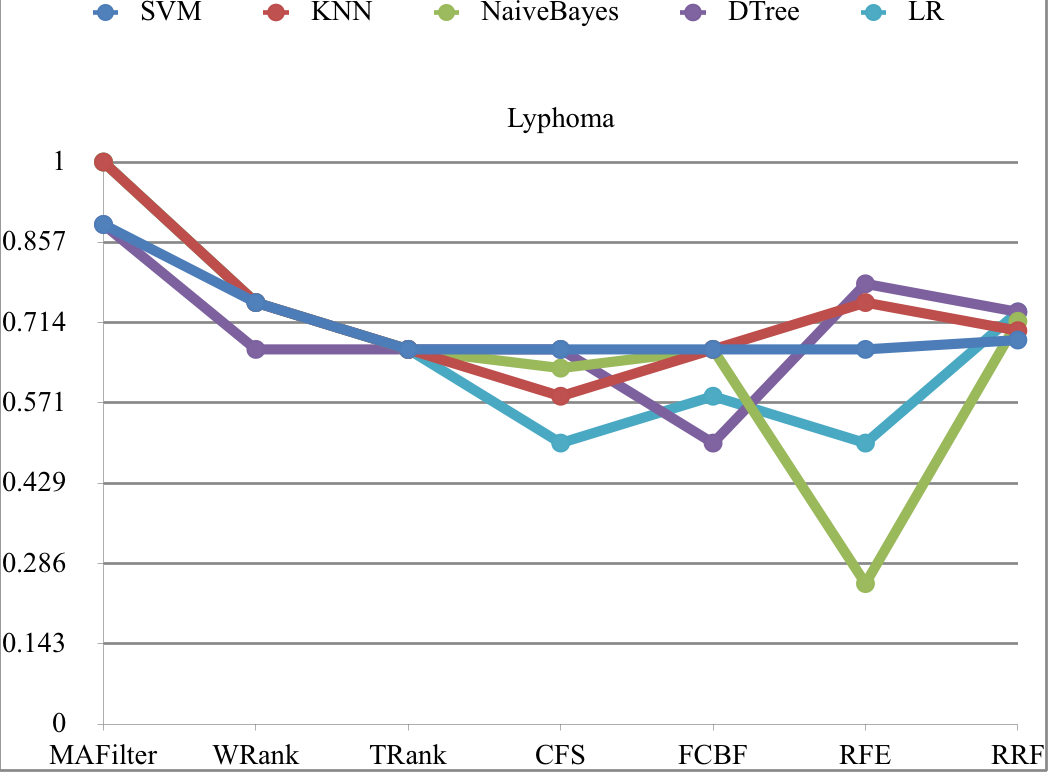
\includegraphics[width=5in]{pic/fig7}, 
  \caption{Lyphoma结果比较}
\end{figure}

\begin{figure}[!ht]
  \centering
  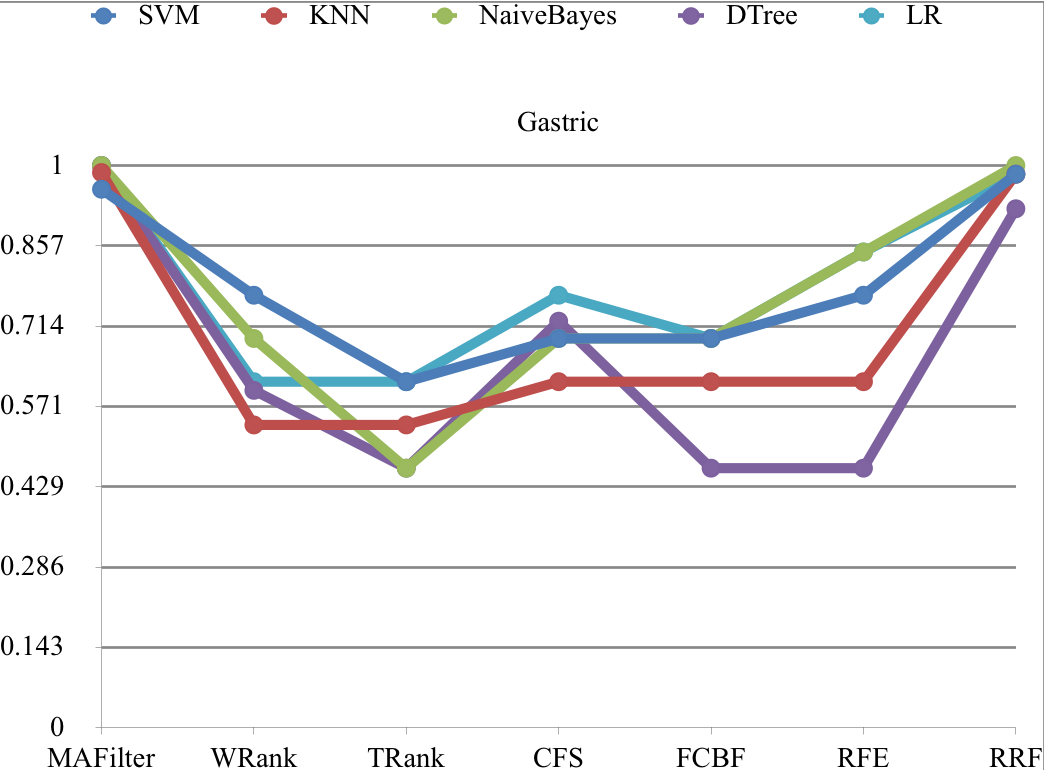
\includegraphics[width=5in]{pic/fig8}, 
  \caption{Gastric结果比较}
\end{figure}

\begin{figure}[!ht]
  \centering
  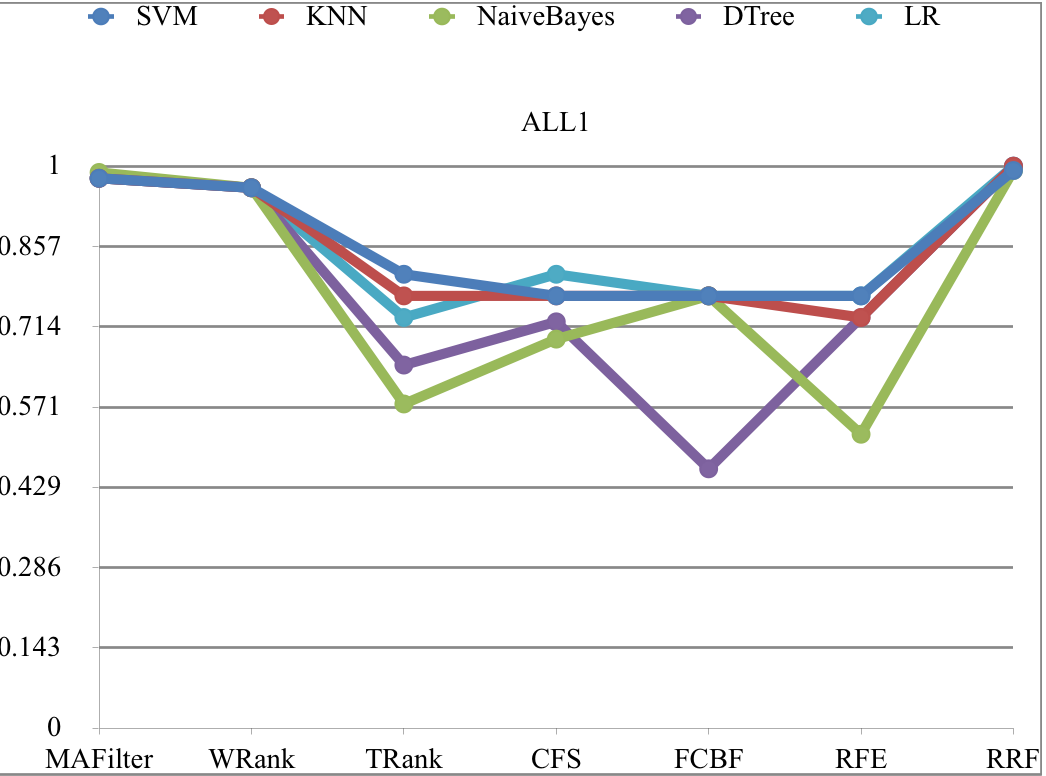
\includegraphics[width=5in]{pic/fig9}, 
  \caption{ALL1结果比较}
\end{figure}

\begin{figure}[!ht]
  \centering
  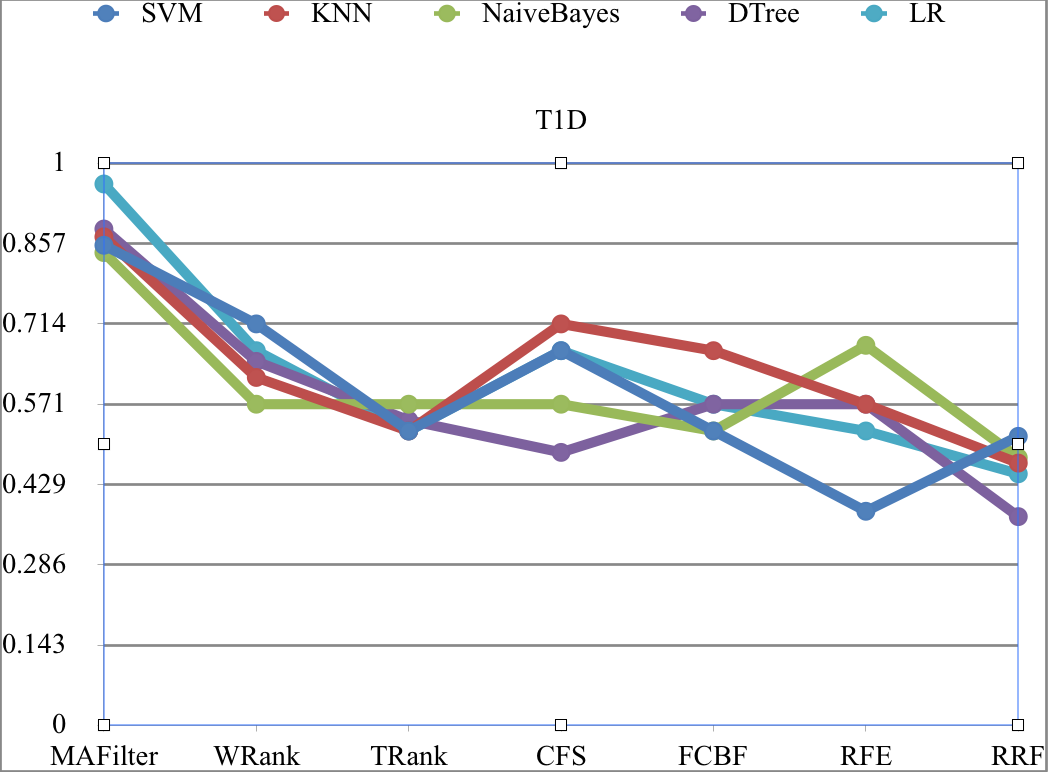
\includegraphics[width=5in]{pic/fig10}, 
  \caption{T1D结果比较}
\end{figure}

\begin{figure}[!ht]
  \centering
  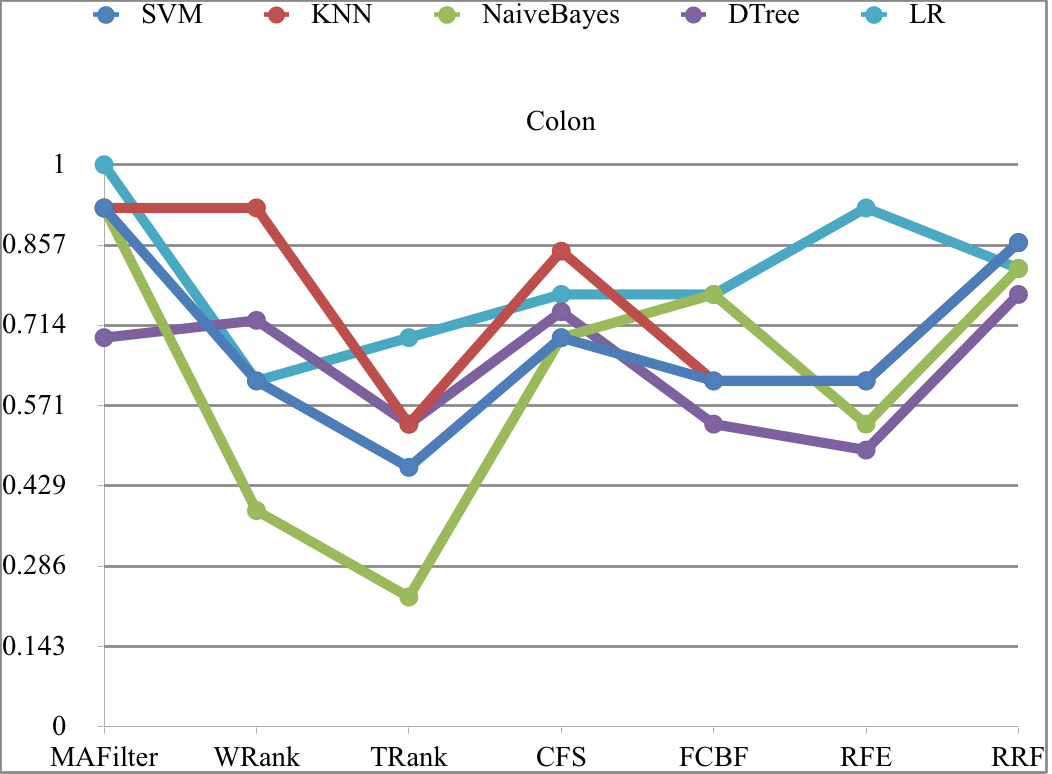
\includegraphics[width=5in]{pic/fig11}, 
  \caption{Colon结果比较}
\end{figure}

\begin{figure}[!ht]
  \centering
  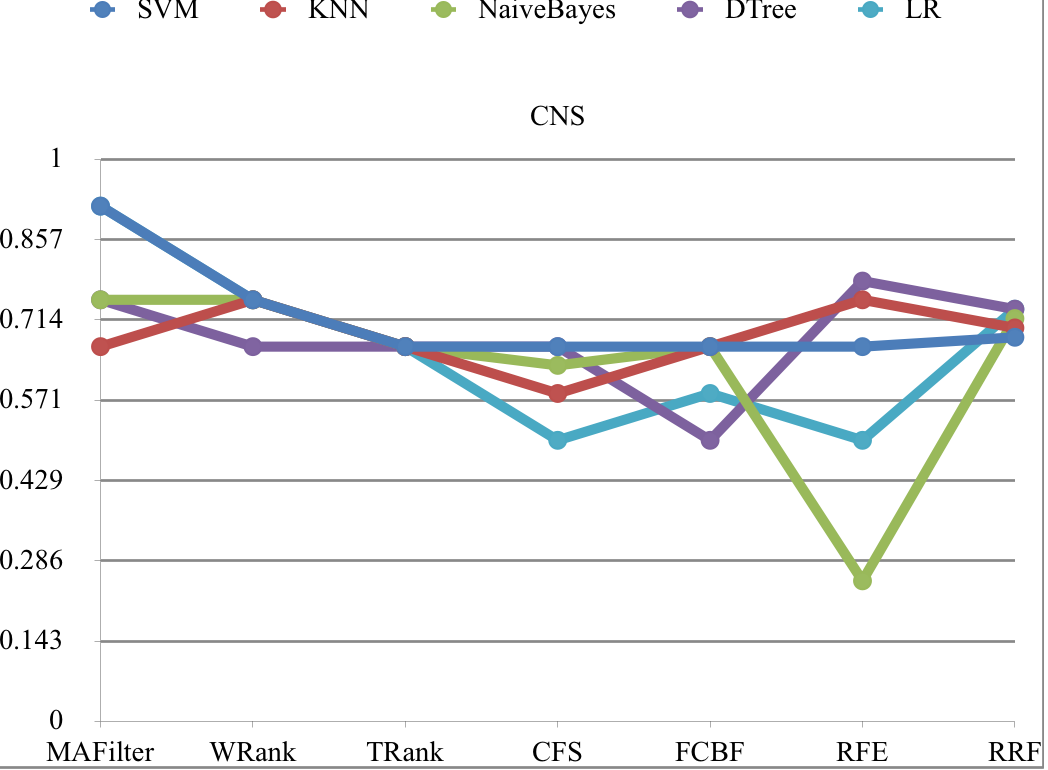
\includegraphics[width=5in]{pic/fig12}, 
  \caption{CNS结果比较}
\end{figure}

\begin{table}        
\centering
\caption{Lymphoma数据集实验结果}
\begin{tabular}{cccccc}
\hline
  & SVM & KNN & NaiveBayes & DTree & LR\\
\hline
MAFilter&	0.888889&	1.000000	&1.000000	&0.888889&	1.000000\\
WRank	&0.750000&	0.750000	&0.750000	&0.666667	&0.750000\\
TRank&	0.666667	&0.666667&	0.666667	&0.666667&	0.666667\\
CFS&	0.666667	&0.583333	&0.633333&	0.666667&	0.500000\\
FCBF&	0.666667&	0.666667	&0.666667	&0.500000	&0.583333\\
RFE	&0.666667	&0.750000&	0.250000&	0.783333&	0.500000\\
RRF	&0.683333&	0.700000&	0.716667&	0.733333&	0.733333\\
\hline
\end{tabular}
\end{table}


\begin{table}        
\centering
\caption{Gastric数据集实验结果}
\begin{tabular}{cccccc}
\hline
  & SVM & KNN & NaiveBayes & DTree & LR\\
\hline
MAFilter&	0.957812&	0.987523&	1.000000&	1.000000&	1.000000\\
WRank	&0.769231&	0.538462&	0.692308&	0.600000	&0.615385\\
TRank	&0.615385&	0.538462&	0.461538&	0.461538&	0.615385\\
CFS	&0.692308&	0.615385&	0.692308&	0.723077	&0.769231\\
FCBF&	0.692308&	0.615385&	0.692308&	0.461538&	0.692308\\
RFE&	0.769231&	0.615385&	0.846150&	0.461538&	0.846154\\
RRF&	0.984615&	0.984615&	1.000000&	0.923077&	0.984615\\
\hline
\end{tabular}
\end{table}

\begin{table}        
\centering
\caption{ALL1数据集实验结果}
\begin{tabular}{cccccc}
\hline
  & SVM & KNN & NaiveBayes & DTree & LR\\
\hline
MAFilter&	0.978545&	0.978545&	0.988889&	0.978545&	0.978545\\
WRank	&0.961538&	0.961538&	0.961538&	0.961538&	0.961538\\
TRank	&0.807692&	0.769231&	0.576923&	0.646154&	0.730769\\
CFS	&0.769231	&0.769231&	0.692308	&0.723077&	0.807692\\
FCBF&	0.769231&	0.769231&	0.769231&	0.461538&	0.769231\\
RFE&	0.769231&	0.730769&	0.523077&	0.730769&	0.769231\\
RRF&	0.992308&	1.000000&	0.992308&	1.000000&	1.000000\\
\hline
\end{tabular}
\end{table}

\begin{table}        
\centering
\caption{T1D数据集实验结果}
\begin{tabular}{cccccc}
\hline
  & SVM & KNN & NaiveBayes & DTree & LR\\
\hline
MAFilter&0.854230&	0.869212&	0.841234&	0.883132&	0.963260\\
WRank&	0.714286&	0.619048&	0.571429&	0.647619&	0.666667\\
TRank&	0.523810&	0.523810&	0.571429&	0.542857&	0.523810\\
CFS&	0.666667&	0.714286&	0.571429&	0.485714&	0.666667\\
FCBF&	0.523810&	0.666667&	0.523810&	0.571429&	0.571429\\
RFE&	0.380952&	0.571429&	0.676190&	0.571429&	0.523810\\
RRF&	0.514286&	0.466667&	0.476190&	0.371429&	0.447619\\
\hline
\end{tabular}
\end{table}

\begin{table}        
\centering
\caption{Colon数据集实验结果}
\begin{tabular}{cccccc}
\hline
  & SVM & KNN & NaiveBayes & DTree & LR\\
\hline
MAFilter&0.923077&	0.923077&	0.923077&	0.692308&	1\\
WRank&	0.615385&	0.923077&	0.384615&	0.723077&	0.615385\\
TRank&	0.461538&	0.538462&	0.230769&	0.538462&	0.692308\\
CFS&	0.692308&	0.846154&	0.692308&	0.738462&	0.769231\\
FCBF&	0.615385&	0.615385&	0.769231&	0.538462&	0.769231\\
RFE&	0.615385&	0.615385&	0.538462&	0.492308&	0.923077\\
RRF&	0.861538&	0.861530&	0.815385&	0.769231&	0.815385\\
\hline
\end{tabular}
\end{table}

\begin{table}        
\centering
\caption{CNS数据集实验结果}
\begin{tabular}{cccccc}
\hline
  & SVM & KNN & NaiveBayes & DTree & LR\\
\hline
MAFilter&0.916667&	0.666667&	0.750000&	0.750000&	0.916667\\
WRank&	0.750000&	0.750000&	0.750000&	0.666667&	0.750000\\
TRank&	0.666667&	0.666667&	0.666667&	0.666667&	0.666667\\
CFS&	0.666667&	0.583333&	0.633333&	0.666667&	0.500000\\
FCBF&	0.666667&	0.666667&	0.666667&	0.500000&	0.583333\\
RFE&	0.666667&	0.750000&	0.250000&	0.783333&	0.500000\\
RRF&	0.683333&	0.700000&	0.716667&	0.733333&	0.733333\\  
\hline
\end{tabular}
\end{table}



\end{document}
